\documentclass{standalone}
\usepackage{tikz}
\usetikzlibrary{patterns, positioning}


\begin{document}
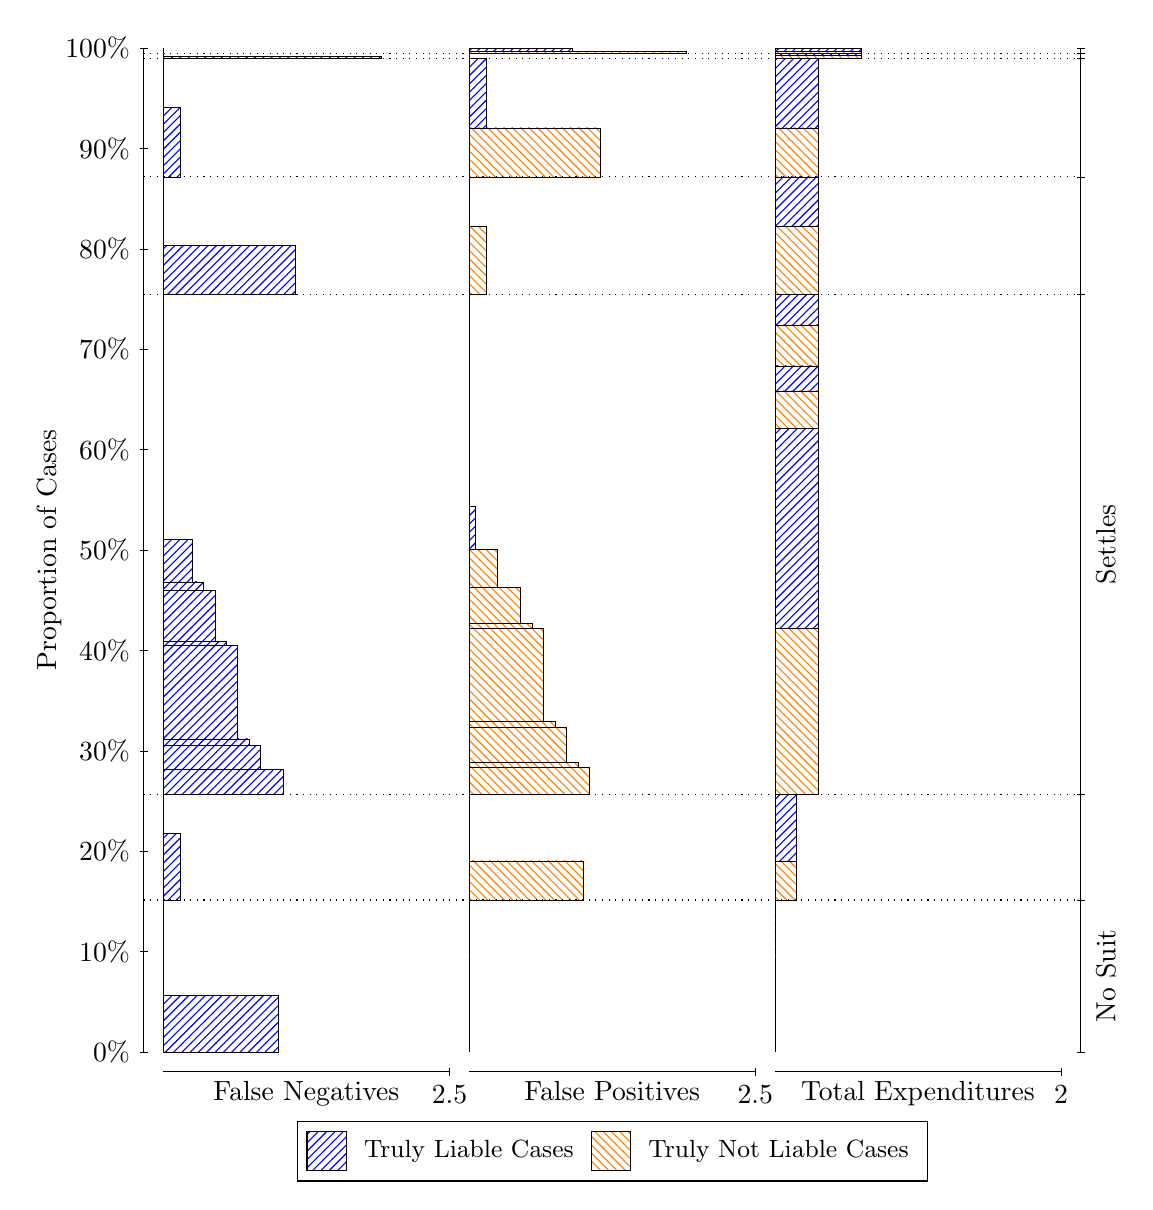
\begin{tikzpicture}
\draw[black, very thin] (1.5,1.75) -- (1.5,14.5);
\node[rotate=90, text=black, anchor=center] at (0.3, 8.125) {Proportion of Cases};
\draw[black, very thin] (1.45,1.75) -- (1.55,1.75);
\node[text=black, anchor=east] at (1.45, 1.75) {0\%};
\draw[black, very thin] (1.45,3.025) -- (1.55,3.025);
\node[text=black, anchor=east] at (1.45, 3.025) {10\%};
\draw[black, very thin] (1.45,4.3) -- (1.55,4.3);
\node[text=black, anchor=east] at (1.45, 4.3) {20\%};
\draw[black, very thin] (1.45,5.575) -- (1.55,5.575);
\node[text=black, anchor=east] at (1.45, 5.575) {30\%};
\draw[black, very thin] (1.45,6.85) -- (1.55,6.85);
\node[text=black, anchor=east] at (1.45, 6.85) {40\%};
\draw[black, very thin] (1.45,8.125) -- (1.55,8.125);
\node[text=black, anchor=east] at (1.45, 8.125) {50\%};
\draw[black, very thin] (1.45,9.4) -- (1.55,9.4);
\node[text=black, anchor=east] at (1.45, 9.4) {60\%};
\draw[black, very thin] (1.45,10.675) -- (1.55,10.675);
\node[text=black, anchor=east] at (1.45, 10.675) {70\%};
\draw[black, very thin] (1.45,11.95) -- (1.55,11.95);
\node[text=black, anchor=east] at (1.45, 11.95) {80\%};
\draw[black, very thin] (1.45,13.225) -- (1.55,13.225);
\node[text=black, anchor=east] at (1.45, 13.225) {90\%};
\draw[black, very thin] (1.45,14.5) -- (1.55,14.5);
\node[text=black, anchor=east] at (1.45, 14.5) {100\%};

\draw[black, very thin] (13.4,1.75) -- (13.4,14.5);
\draw[black, very thin] (13.35,1.75) -- (13.45,1.75);
\node[anchor=west] at (13.35, 1.75) {};
\draw[black, very thin] (13.35,3.6806) -- (13.45,3.6806);
\node[anchor=west] at (13.35, 3.6806) {};
\draw[black, very thin] (13.35,5.0219) -- (13.45,5.0219);
\node[anchor=west] at (13.35, 5.0219) {};
\draw[black, very thin] (13.35,11.373) -- (13.45,11.373);
\node[anchor=west] at (13.35, 11.373) {};
\draw[black, very thin] (13.35,12.864) -- (13.45,12.864);
\node[anchor=west] at (13.35, 12.864) {};
\draw[black, very thin] (13.35,14.37) -- (13.45,14.37);
\node[anchor=west] at (13.35, 14.37) {};
\draw[black, very thin] (13.35,14.433) -- (13.45,14.433);
\node[anchor=west] at (13.35, 14.433) {};
\draw[black, very thin] (13.35,14.5) -- (13.45,14.5);
\node[anchor=west] at (13.35, 14.5) {};

\draw[black, very thin, pattern color=blue, pattern=north east lines] (1.75,1.75) rectangle (3.2033,2.4685);
\draw[black, very thin, pattern color=orange, pattern=north west lines] (1.75,2.4685) rectangle (1.75,3.6806);
\draw[black, very thin, pattern color=blue, pattern=north east lines] (1.75,3.6806) rectangle (1.968,4.5267);
\draw[black, very thin, pattern color=orange, pattern=north west lines] (1.75,4.5267) rectangle (1.75,5.0219);
\draw[black, very thin, pattern color=blue, pattern=north east lines] (1.75,5.0219) rectangle (3.276,5.338);
\draw[black, very thin, pattern color=blue, pattern=north east lines] (1.75,5.338) rectangle (2.9853,5.6447);
\draw[black, very thin, pattern color=blue, pattern=north east lines] (1.75,5.6447) rectangle (2.84,5.7252);
\draw[black, very thin, pattern color=blue, pattern=north east lines] (1.75,5.7252) rectangle (2.6947,6.9118);
\draw[black, very thin, pattern color=blue, pattern=north east lines] (1.75,6.9118) rectangle (2.5493,6.9685);
\draw[black, very thin, pattern color=blue, pattern=north east lines] (1.75,6.9685) rectangle (2.404,7.6144);
\draw[black, very thin, pattern color=blue, pattern=north east lines] (1.75,7.6144) rectangle (2.2587,7.7194);
\draw[black, very thin, pattern color=blue, pattern=north east lines] (1.75,7.7194) rectangle (2.1133,8.2581);
\draw[black, very thin, pattern color=orange, pattern=north west lines] (1.75,8.2581) rectangle (1.75,11.373);
\draw[black, very thin, pattern color=blue, pattern=north east lines] (1.75,11.373) rectangle (3.4213,11.998);
\draw[black, very thin, pattern color=orange, pattern=north west lines] (1.75,11.998) rectangle (1.75,12.864);
\draw[black, very thin, pattern color=blue, pattern=north east lines] (1.75,12.864) rectangle (1.968,13.747);
\draw[black, very thin, pattern color=orange, pattern=north west lines] (1.75,13.747) rectangle (1.75,14.37);
\draw[black, very thin, pattern color=blue, pattern=north east lines] (1.75,14.37) rectangle (4.5113,14.397);
\draw[black, very thin, pattern color=orange, pattern=north west lines] (1.75,14.397) rectangle (1.75,14.433);
\draw[black, very thin, pattern color=orange, pattern=north west lines] (1.75,14.433) rectangle (1.75,14.462);
\draw[black, very thin, pattern color=blue, pattern=north east lines] (1.75,14.462) rectangle (1.75,14.5);
\draw[black, very thin, pattern color=orange, pattern=north west lines] (5.6333,1.75) rectangle (5.6333,2.9621);
\draw[black, very thin, pattern color=blue, pattern=north east lines] (5.6333,2.9621) rectangle (5.6333,3.6806);
\draw[black, very thin, pattern color=orange, pattern=north west lines] (5.6333,3.6806) rectangle (7.0867,4.1758);
\draw[black, very thin, pattern color=blue, pattern=north east lines] (5.6333,4.1758) rectangle (5.6333,5.0219);
\draw[black, very thin, pattern color=orange, pattern=north west lines] (5.6333,5.0219) rectangle (7.1593,5.3686);
\draw[black, very thin, pattern color=orange, pattern=north west lines] (5.6333,5.3686) rectangle (7.014,5.4282);
\draw[black, very thin, pattern color=orange, pattern=north west lines] (5.6333,5.4282) rectangle (6.8687,5.8683);
\draw[black, very thin, pattern color=orange, pattern=north west lines] (5.6333,5.8683) rectangle (6.7233,5.9459);
\draw[black, very thin, pattern color=orange, pattern=north west lines] (5.6333,5.9459) rectangle (6.578,7.1319);
\draw[black, very thin, pattern color=orange, pattern=north west lines] (5.6333,7.1319) rectangle (6.4327,7.1946);
\draw[black, very thin, pattern color=orange, pattern=north west lines] (5.6333,7.1946) rectangle (6.2873,7.6551);
\draw[black, very thin, pattern color=orange, pattern=north west lines] (5.6333,7.6551) rectangle (5.9967,8.1365);
\draw[black, very thin, pattern color=blue, pattern=north east lines] (5.6333,8.1365) rectangle (5.706,8.6753);
\draw[black, very thin, pattern color=blue, pattern=north east lines] (5.6333,8.6753) rectangle (5.6333,11.373);
\draw[black, very thin, pattern color=orange, pattern=north west lines] (5.6333,11.373) rectangle (5.8513,12.239);
\draw[black, very thin, pattern color=blue, pattern=north east lines] (5.6333,12.239) rectangle (5.6333,12.864);
\draw[black, very thin, pattern color=orange, pattern=north west lines] (5.6333,12.864) rectangle (7.3047,13.487);
\draw[black, very thin, pattern color=blue, pattern=north east lines] (5.6333,13.487) rectangle (5.8513,14.37);
\draw[black, very thin, pattern color=orange, pattern=north west lines] (5.6333,14.37) rectangle (5.6333,14.405);
\draw[black, very thin, pattern color=blue, pattern=north east lines] (5.6333,14.405) rectangle (5.6333,14.433);
\draw[black, very thin, pattern color=orange, pattern=north west lines] (5.6333,14.433) rectangle (8.3947,14.462);
\draw[black, very thin, pattern color=blue, pattern=north east lines] (5.6333,14.462) rectangle (6.9413,14.5);
\draw[black, very thin, pattern color=orange, pattern=north west lines] (9.5167,1.75) rectangle (9.5167,2.9621);
\draw[black, very thin, pattern color=blue, pattern=north east lines] (9.5167,2.9621) rectangle (9.5167,3.6806);
\draw[black, very thin, pattern color=orange, pattern=north west lines] (9.5167,3.6806) rectangle (9.7892,4.1758);
\draw[black, very thin, pattern color=blue, pattern=north east lines] (9.5167,4.1758) rectangle (9.7892,5.0219);
\draw[black, very thin, pattern color=orange, pattern=north west lines] (9.5167,5.0219) rectangle (10.062,7.1319);
\draw[black, very thin, pattern color=blue, pattern=north east lines] (9.5167,7.1319) rectangle (10.062,9.6648);
\draw[black, very thin, pattern color=orange, pattern=north west lines] (9.5167,9.6648) rectangle (10.062,10.146);
\draw[black, very thin, pattern color=blue, pattern=north east lines] (9.5167,10.146) rectangle (10.062,10.462);
\draw[black, very thin, pattern color=orange, pattern=north west lines] (9.5167,10.462) rectangle (10.062,10.985);
\draw[black, very thin, pattern color=blue, pattern=north east lines] (9.5167,10.985) rectangle (10.062,11.373);
\draw[black, very thin, pattern color=orange, pattern=north west lines] (9.5167,11.373) rectangle (10.062,12.239);
\draw[black, very thin, pattern color=blue, pattern=north east lines] (9.5167,12.239) rectangle (10.062,12.864);
\draw[black, very thin, pattern color=orange, pattern=north west lines] (9.5167,12.864) rectangle (10.062,13.487);
\draw[black, very thin, pattern color=blue, pattern=north east lines] (9.5167,13.487) rectangle (10.062,14.37);
\draw[black, very thin, pattern color=orange, pattern=north west lines] (9.5167,14.37) rectangle (10.607,14.405);
\draw[black, very thin, pattern color=blue, pattern=north east lines] (9.5167,14.405) rectangle (10.607,14.433);
\draw[black, very thin, pattern color=orange, pattern=north west lines] (9.5167,14.433) rectangle (10.607,14.462);
\draw[black, very thin, pattern color=blue, pattern=north east lines] (9.5167,14.462) rectangle (10.607,14.5);
\draw[black, dotted] (1.5,3.6806) -- (13.4,3.6806);
\draw[black, dotted] (1.5,5.0219) -- (13.4,5.0219);
\draw[black, dotted] (1.5,11.373) -- (13.4,11.373);
\draw[black, dotted] (1.5,12.864) -- (13.4,12.864);
\draw[black, dotted] (1.5,14.37) -- (13.4,14.37);
\draw[black, dotted] (1.5,14.433) -- (13.4,14.433);
\draw[black, very thin] (1.75,1.5) -- (5.3833,1.5);
\node[text=black, anchor=north] at (3.5667, 1.5) {False Negatives};
\draw[black, very thin] (5.3833,1.45) -- (5.3833,1.55);
\node[text=black, anchor=north] at (5.3833, 1.45) {2.5};

\draw[black, very thin] (5.6333,1.5) -- (9.2667,1.5);
\node[text=black, anchor=north] at (7.45, 1.5) {False Positives};
\draw[black, very thin] (9.2667,1.45) -- (9.2667,1.55);
\node[text=black, anchor=north] at (9.2667, 1.45) {2.5};

\draw[black, very thin] (9.5167,1.5) -- (13.15,1.5);
\node[text=black, anchor=north] at (11.333, 1.5) {Total Expenditures};
\draw[black, very thin] (13.15,1.45) -- (13.15,1.55);
\node[text=black, anchor=north] at (13.15, 1.45) {2};

\node[text=black, centered, rotate=90] at (13.72, 2.7153) {No Suit};

\node[text=black, centered, rotate=90] at (13.72, 8.1973) {Settles};





\draw (7.449999999999999,1.5) node[draw=none] (baseCoordinate) {};
\begin{scope}[align=center]
        \matrix[scale=0.5, draw=black, below=0.5cm of baseCoordinate, nodes={draw}, column sep=0.1cm]{
            \node[rectangle, draw, minimum width=0.5cm, minimum height=0.5cm, pattern color=blue, pattern=north east lines] {}; &
            \node[draw=none, font=\small, text=black] (B) {Truly Liable Cases}; &
            \node[rectangle, draw, minimum width=0.5cm, minimum height=0.5cm, pattern color=orange, pattern=north west lines] {}; &
            \node[draw=none, font=\small, text=black] (B) {Truly Not Liable Cases}; \\
            };
\end{scope}

\end{tikzpicture}
\end{document}